% !TeX root = ../thuthesis-example.tex

\chapter{引言}
\section{研究背景\label{sec:chap1-sec1}}
“物联网”这一术语通常指的是将网络的连接性和计算能力拓展到通常不被视为计算机的物体、传感器和日常物品,使这些设备能够在最小的人工干预下生成、交换和消费数据。物联网这一词汇最早由英国人 Kevin Ashton 在 1999 年用于描述一个系统,在该系统中,物理世界中的对象通过传感器连接到互联网\cite{li2015internet}。一些预测认为,到 2025 年,全球参与物联网的设备数可能达到 1000 亿台,对经济的影响超过 11 万亿美元\cite{rose2015internet}。

在 2013 年德国汉诺威工业展览会上,“工业 4.0”理念首度面世\cite{ghobakhloo2020industry},其中提及的工业物联网(Industrial Internet of Things, IIoT)在全球范围内引起了广泛关注。IIoT 关注将所有的工业资产,包括及其和控制系统,与信息系统和业务流程连接起来,从中收集的大量数据可以为工业生产、管理、解决方案设计提供重要的参考作用\cite{sisinni2018industrial}。工业物联网会产生大量工业数据,其类型包括时间序列、图片、视频、文档等,在某些场景下一年内甚至会产生 $4\times 10^{12}$ GB 数据\cite{ge2012riseofindustrial}。在这些数据中,时间序列数据主要由机器设备上的传感器采集产生,由于采集频率高、传感器数量多,成为了工业大数据的主体\cite{di2019industrial}。

工业物联网场景下传感器数量可能很多,写入数据的速率也很高。例如,一架波音 787 客机在一次飞行中就可以产生超过 512 GB 的时序数据\cite{ronkainen2015designing};上海地铁目前有 136 列地铁的传感器数据开始被收集和监控,一年产生的数据量超过 254 TB;长安汽车集团生产的每一辆汽车上均有数千个传感器,其车联网应用一共管理了近 12 亿条时间序列,每年产生的数据量超过 13,000 TB。

海量的时序数据对数据的写入、存储和查询都提出了挑战。传统的关系型数据库通常使用 B+ 树作为底层的存储数据结构,其在处理点写入、点查询等负载时具有较好的性能,但是在面对工业物联网场景下时序数据的高速率写入和聚合查询负载时性能较差,无法满足需求\cite{jensen2017time}。因此,一种专门为存储时序数据而设计的数据库应运而生,它们被称为时序数据库(Time Series Database,TSDB)。如图 \ref{fig:db-engine} 所示,在国际权威数据库流行度排行机构 DB-Engines 的调查结果中,时序数据库在过去十年内的流行度持续上升,目前其流行度仅次于图数据库,位居榜单中的第二名。

\begin{figure}
  \centering
  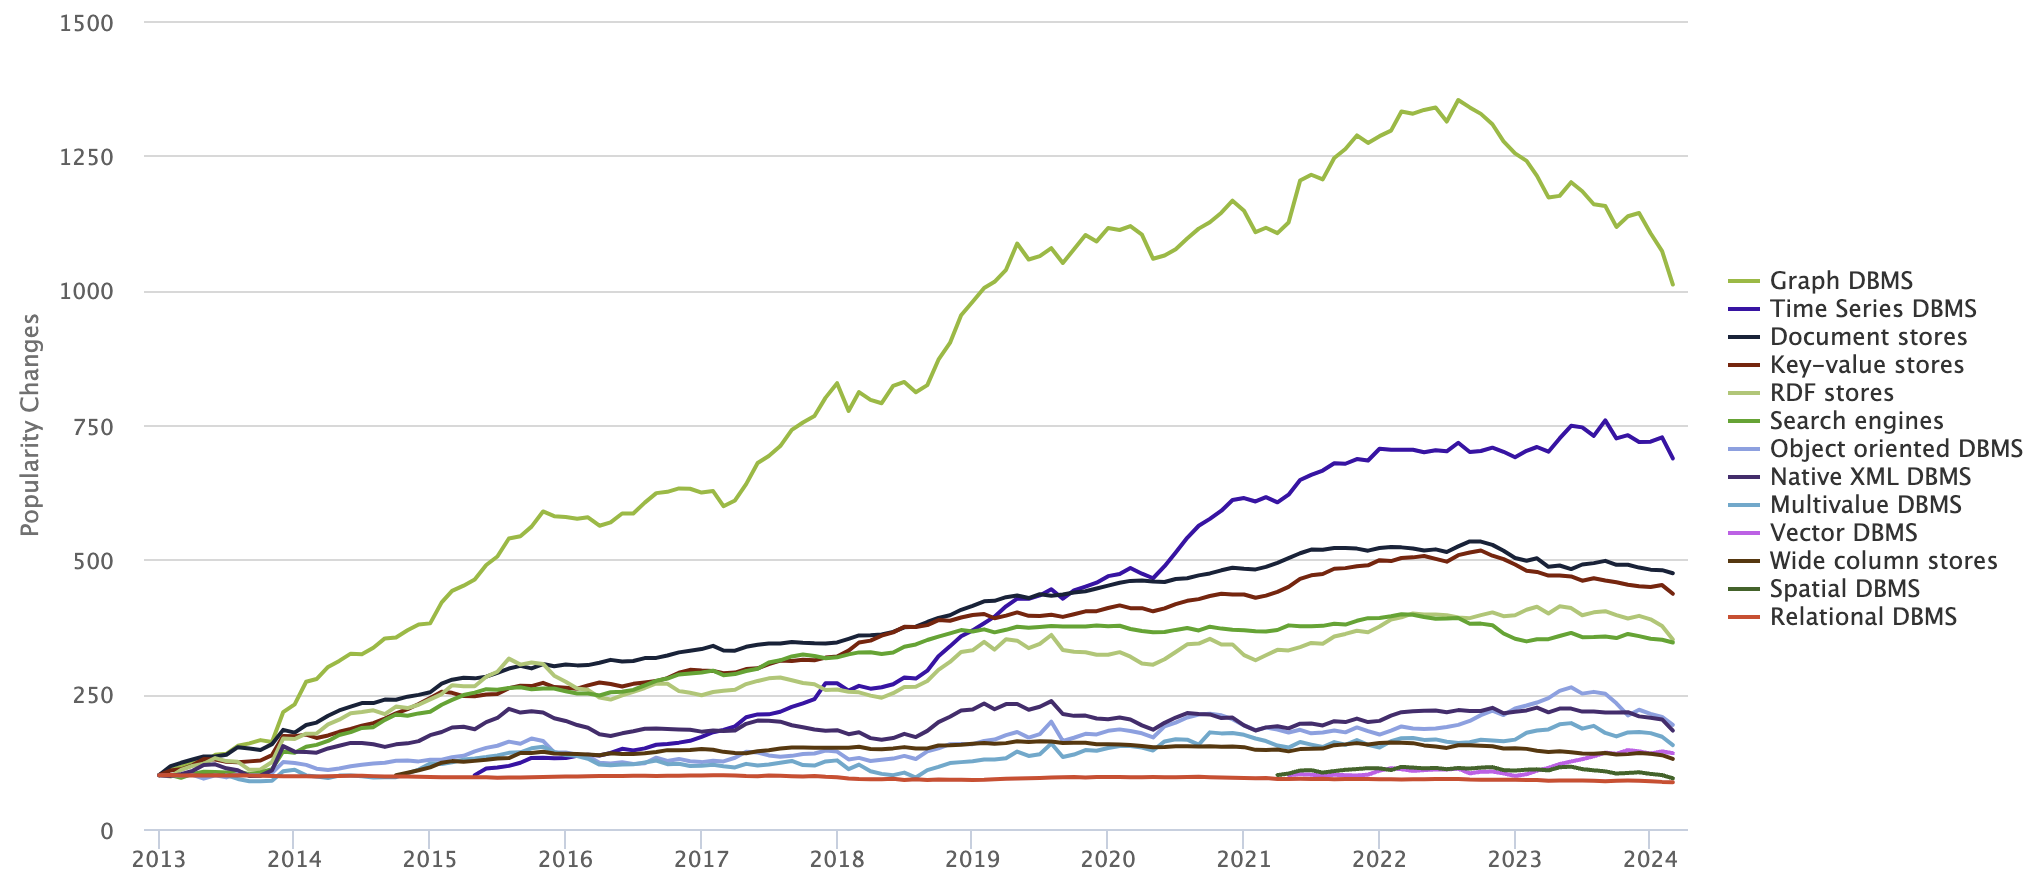
\includegraphics[width=\linewidth]{db-engines-ranking.png}
  \caption{DB-Engine 数据库类型流行度排名}
  \label{fig:db-engine}
\end{figure}

Apache IoTDB 是 Apache 基金会下一款开源的时序数据库,其具有为时间序列数据所优化的存储引擎、查询引擎以及分布式框架,可以满足工业物联网领域对海量时间序列数据高速写入、存储、快速读取以及复杂查询的需求\cite{wang2023apache}。

针对工业物联网场景下大量时序数据高速写入的需求,Apache IoTDB 主要提供了三种类型的数据写入接口:SQL 写入、原生列式写入接口、原生行式写入接口。在写入性能上,原生列式写入接口的性能最优,原生行式写入接口次之,SQL 写入性能最差;在写入的灵活性上,SQL 写入的灵活性最高,原生行式写入接口的灵活性次之,原生列式写入接口的灵活性最差。在大部分用户的使用场景中,SQL 式写入性能难以满足要求,原生列式写入接口则灵活性不足,使用原生行式写入接口可以兼具灵活性和良好的性能。但是,随着时序数据体量越来越大,原生行式接口写入较列式写入性能较差的问题显得越来越重要。例如,长安汽车车联网项目的一期工程有 12 亿条时间序列,采样周期为 30 秒,而二期工程不仅有 80 亿条时间序列,采样周期也减小到了 10 秒。如果原生行式写入接口的性能不变,粗略估计二期工程的服务器硬件成本约为一期的 20 倍。如果可以重新设计和实现一套高性能的行式写入机制,在负载相同的情况下就可以帮助用户降低机器的硬件成本,在负载越大的场景降成本的效果就越明显。设计和实现一套高性能的行式写入机制需要对客户端、网络传输、存储引擎等组件进行精心的设计和细致的优化。因此,提高 IoTDB 行式写入的性能具有一定的挑战性以及重要的实际意义和应用价值。
\section{Apache IoTDB 现有行式写入机制分析\label{sec:chap1-sec2}}
\subsection{Apache IoTDB 行式写入接口定义}
在 Apache IoTDB 中,时间序列采用树形的元数据结构进行描述。例如,某条时间序列可以被描述为 root.sg.d.s1,该字符串由多个“.”分隔开,“.”之间的字符则为元数据树中的一个节点。一条时间序列都倒数第二个节点被称为一个设备(Device),例如在前面的例子中 root.sg.d 就是一个设备。如果两个或多个时间序列都设备相同,那么则称这些时间序列是同一个设备下的序列。在大部分用户建模的场景中,设备通常对应了现实中的一个实体,例如一台机器或者一辆汽车,而设备下的每条序列则对应实体上部署的传感器。

IoTDB 提供的原生行式写入接口为 insertRecord 和 insertRecords,前者一次发送一行记录,而后者一次发送多行记录。为了减少由于网络传输带来的开销,大部分用户选择使用后者进行写入,本文所关注和研究的对象也主要是后者,即一次发送多行记录的写入形式。以 IoTDB 的 Java 客户端为例,insertRecord 和 insertRecords 接口的定义为:
\begin{lstlisting}[language=java,frame = trBL , firstnumber = last , escapeinside={(*@}{@*)}]
  void insertRecord(
      String deviceId,
      long time,
      List<String> measurements,
      List<TSDataType> types,
      List<Object> values
      )

  void insertRecords(
      List<String> deviceIds, 
      List<Long> times, 
      List<List<String>> measurementsList, 
      List<List<TSDataType>> typesList, 
      List<List<Object>> valuesList
      )
\end{lstlisting}
insertRecord 一次发送一行记录,这里的一行记录指的是这些数据属于一个设备下的时间序列,并且这些数据的时间戳都是相同的。表 \ref{tabular:insert-record-params} 详细介绍了该接口每个参数的含义。
\begin{table}
  \centering
  \caption{insertRecord 参数说明}
  \begin{tabular}{lll}
    \toprule
    参数名 &  类型 & 描述 \\
    \midrule
    deviceId & String & 数据所属的设备 ID \\
    time & long & 数据的时间戳 \\
    measurements & List<String> & 每个数据点所属的时间序列 ID 组成的列表 \\
    types & List<TSDataType> & 每个数据点所对应的数据类型 \\
    values & List<Object> & 每个数据点的数据 \\
    \bottomrule
  \end{tabular}
  \label{tabular:insert-record-params}
\end{table}

insertRecords 接口实际上是把多行记录一起从客户端发送到服务器,从接口的定义上看,每个与 insertRecord 接口对应的参数都变成了对应的列表,列表中的一个元素就描述了对应记录的相关信息,例如 deviceIds 中的每个元素就是每行记录对应的设备 ID。表\ref{tabular:insert-records-params} 中描述了 insertRecords 每个参数的含义。

\begin{table}
  \centering
  \caption{insertRecords 参数说明}
  \begin{tabular}{lll}
    \toprule
    参数名 &  类型 & 描述 \\
    \midrule
    deviceIds & List<String> & 每行记录所属的设备 ID 组成的列表 \\
     times & List<Long> & 每行记录的时间戳组成的列表 \\
    measurementsList & List<List<String> > & 每行记录的序列 ID 列表组成的列表 \\
    typesList & List<List<TSDataType> > & 每行记录数据类型列表组成的列表 \\
    valuesList & List<List<Object> > & 每行记录值列表组成的列表 \\
    \bottomrule
  \end{tabular}
  \label{tabular:insert-records-params}
\end{table}

综上,IoTDB 原生行式写入接口可以一次写入若干行记录,每条记录包含一个设备在一个时间戳下一条或若干条时间序列的数值。
\subsection{Apache IoTDB 现有行式写入机制实现}
如图\ref{fig:iotdb-write-process}所示,目前 Apache IoTDB 的行式写入流程主要分为三个阶段:
\begin{enumerate}
  \item \textbf{客户端侧数据预处理}。此阶段从客户端的行式写入函数被用户调用开始,到客户端调用远程过程调用层的数据发送方法前结束。这个阶段进行的工作是校验用户传入的参数是否合法,检验客户端状态,选取合适的服务器节点作为数据发送的目标(在分布式部署时可能存在多个服务器节点),对数据进行部分序列化。
  \item \textbf{远程过程调用层数据传输}。远程过程调用(Remote Procedure Call,RPC)层跨越了客户端侧和服务器侧,其负责的主要工作为:将客户端侧传入的数据根据预定义的结构序列化为二进制的数据流,并通过网络传输到服务器侧,再反序列化为预定义的数据结构,交由服务器中 IoTDB 上层的处理逻辑完成后续流程。
  \item \textbf{IoTDB 处理写入请求}。此时写入请求被 RPC 层反序列化为预定义的写入请求数据结构,IoTDB 会进行时间序列 ID 和路径校验、元数据校验、权限校验、MPP 框架处理、内存控制处理、监控框架记录性能指标、写预写日志(Write Ahead Log,WAL)、写入内存表、更新内存索引等步骤,将数据记录在内存和磁盘中。这一步结束以后,整个写入请求就被成功执行了。
\end{enumerate}
\begin{figure}
  \centering
  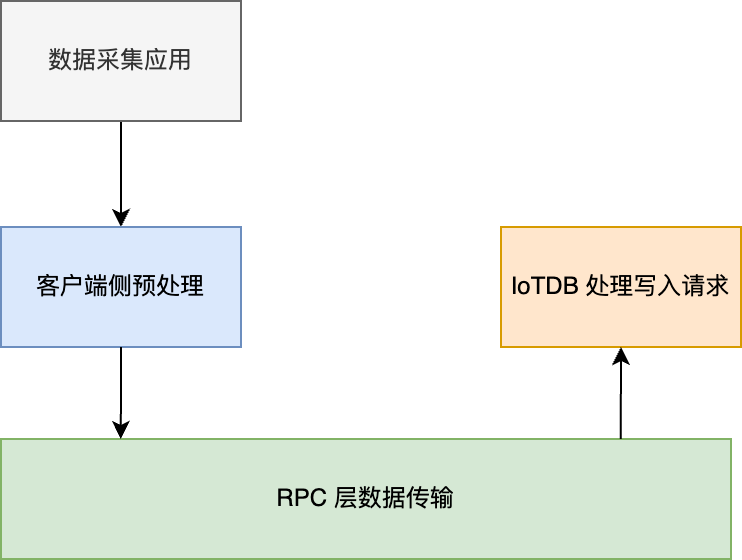
\includegraphics[width=0.7\linewidth]{数据写入整体过程.png}
  \caption{Apache IoTDB 行式写入流程}
  \label{fig:iotdb-write-process}
\end{figure}
\subsection{Apache IoTDB 现有行式写入机制不足}
经过在某些用户场景和压力测试场景下对 Apache IoTDB 的行式写入接口的测试和分析,本文发现目前的实现有以下问题:
\begin{enumerate}
  \item \textbf{服务器侧写入逻辑的实现不够高效}。当一批记录一起到达 IoTDB 的服务端后,目前的实现仍然是逐条进行写入,而不是批量化地写入。这样的实现方式需要对每一行记录都获取写入路径上的多个锁,在监控框架中更新指标,调用很多预处理和后处理函数,这些操作都会带来很大的开销,使得服务器上真正用于记录数据的时间变得很少,资源利用比较低效。
  \item \textbf{RPC 层设计不够合理}。目前 IoTDB 所使用的 RPC 框架是 Apache Thrift,然而目前行式写入接口的实现几乎直接将客户端传入的参数放到了 Thrift 中进行传输。这并没有利用好传入数据的特点,例如不同记录的时间戳范围都比较接近,设备和时间序列 ID 具有一定的相似性。利用这些特点可以对传输的数据进行压缩,减少传输的数据量,提高传输的效率。
  \item \textbf{对客户端侧的资源利用不足}。目前 IoTDB 的客户端侧所执行的工作较为轻量,而将部分与上下文无关的工作,如路径语法校验、内存占用计算等工作留到了服务器侧,这并没有充分利用客户端侧的资源,也没有充分利用客户端侧的计算能力。
\end{enumerate}
由于篇幅原因,对原有行式写入机制不足的详细分析将在后续章节中进一步展开。
\section{研究内容}
结合 \ref{sec:chap1-sec1} 和 \ref{sec:chap1-sec2} 节的分析,本文发现目前 Apache IoTDB 的行式写入接口具有较好的灵活度,但是过去的实现机制在性能上存在一定的不足,在时间序列数较多、写入数据量较大的场景下无法很好地满足用户需求。因此,本工作的研究内容主要包括:
\begin{enumerate}
  \item 如何寻找目前 Apache IoTDB 的不足。目前 IoTDB 的行式写入性能与列式写入性能大约有 2-3 倍的差距,分析这个差距产生的原因并找出目前行式写入机制的设计缺陷和实现缺陷有助于我们在设计新的行式写入机制时避免这些问题。
  \item 如何在保持对原有行式写入接口兼容的情况下设计并实现一套高性能的行式写入机制。由于目前使用 Apache IoTDB 行式写入接口的用户众多,因此在设计新的行式写入机制时需要保持对原有接口的兼容,以减少用户迁移的成本。同时,新的行式写入机制需要从客户端、RPC 层、存储引擎等多个方面进行优化,以提高行式写入的性能。
  \item 如何对 Apache IoTDB 的行式写入机制进行性能评估与分析。设计并实现一套高性能的行式写入机制后,需要对其进行性能评估与分析,以验证其性能的提升效果。目前的性能测试工具并不能很好地反映用户的真实写入场景,因此需要开发一套模拟用户场景的测试工具,收集一些真实用户场景的写入特征,并使用测试工具根据这些特征模拟不同用户的写入场景,验证并分析 Apache IoTDB 行式写入机制的性能。
\end{enumerate}

\section{研究贡献}
本文的主要贡献体现在以下三个方面:
\begin{enumerate}
  \item \textbf{对目前 Apache IoTDB 已有行式写入机制的性能分析}。本工作对目前 Apache IoTDB 的已有行式写入机制进行性能分析,包括对其性能的评估、寻找其性能瓶颈、分析其设计不足等。
  \item \textbf{为 Apache IoTDB 设计并实现一套高性能的行式写入机制}。本工作在吸收目前行式写入机制的优点的基础上,分别对客户端、RPC 层、存储引擎侧进行优化,设计并实现一套高性能的行式写入处理机制,以提高 IoTDB 的行式写入性能。
  \item \textbf{对 Apache IoTDB 的行式写入机制进行性能评估与分析}。本工作开发了一套模拟用户场景的测试工具,收集了一些真实用户场景的写入特征,并使用测试工具根据这些特征模拟不同用户的写入场景,验证并分析 Apache IoTDB 行式写入机制的性能。
\end{enumerate}

\section{本文的组织结构}

本文一共分为九章,每个章节的内容如下:

第 1 章为引言部分,主要介绍了物联网和工业物联网发展背景下时序数据库发展的意义,介绍了 Apache IoTDB 目前的行式写入接口及其具有较好灵活性的优点,并阐述了目前 Apache IoTDB 行式写入机制的不足之处,最后引出了本工作的研究内容和贡献。

第 2 章介绍了相关工作,首先介绍了目前主流数据库及数据湖系统的写入接口,然后介绍了一些高性能存储引擎的设计,最后介绍了目前已有通过优化客户端设计和 RPC 层提高数据库性能的方法。

第 3 章详细介绍了目前 Apache IoTDB 的行式写入机制的运行流程,包括客户端侧的数据预处理、RPC 层的数据传输、IoTDB 服务端的写入处理等,并通过 Arthas 等性能分析工具对这一机制的性能进行了分析,找出了其性能瓶颈,并指出其在设计上和实现上的不足之处,为后文设计新的行式写入机制提供了基础。

第 4 章从整体上介绍了本工作的设计目标和设计思路,包括对客户端、RPC 层、存储引擎的设计思路,以及设计新的行式写入机制的一些原则和约束,为读者对本工作提供一个整体的认识。

第 5 章介绍了对客户端侧的设计和实现,包括对客户端侧的数据预处理、行式写入转列式写入、路径校验、内存开销预计算等方面的设计与实现,并介绍了实现过程中的一些细节。

第 6 章介绍了对 RPC 层的设计和实现,介绍了行式序列化和列式序列化两种 RPC 包设计方案,讨论了这两种方案的优劣,并说明了最终选择列式序列化的原因,最后介绍了 RPC 层的实现细节。

第 7 章介绍了存储引擎侧高性能行式写入机制的设计与实现,包括批量化写入、计划片级并行写入、预写日志优化等。

第 8 章是实验部分,首先介绍了用于模拟用户场景的测试程序的设计,然后介绍了包括中冶赛迪、长安汽车、四维智联等用户的典型写入场景,最后使用模拟测试工具和 IoT-Benchmark\cite{liu2019benchmarking} 两种测试工具对新的行式写入机制进行了性能测试,并对测试结果进行了分析。

第 9 章是总结部分,总结了本文的工作,指出了本文的不足之处,并对未来的工作进行了展望。